\documentclass{VUMIFPSkursinis}
\usepackage{algorithmicx}
\usepackage{algorithm}
\usepackage{algpseudocode}
\usepackage{amsfonts}
\usepackage{amsmath}
\usepackage{bm}
\usepackage{caption}
\usepackage{color}
\usepackage{float}
\usepackage{graphicx}
\usepackage{listings}
\usepackage{subfig}
\usepackage{wrapfig}
\usepackage{lithuanian}
\usepackage{longtable}

\usepackage{enumitem}
\usepackage[lithuanian,german]{babel} 
\usepackage{csquotes} 
\MakeOuterQuote{"} 
\selectlanguage{lithuanian}
%PAKEISTA, tarpai tarp sąrašo elementų
\setitemize{noitemsep,topsep=0pt,parsep=0pt,partopsep=0pt}
\setenumerate{noitemsep,topsep=0pt,parsep=0pt,partopsep=0pt}

% Titulinio aprašas
\university{Vilniaus universitetas}
\faculty{Matematikos ir informatikos fakultetas}
\department{Programų sistemų katedra}
\papertype{Kursinis darbas}
\title{Mažos duomenų imties problemos poveikis klasifikacijos tikslumui naudojant dirbtinius neuroninius tinklus}
\titleineng{(The Effect of a Small Dataset Problem on Classification Accuracy Using Artificial Neural Networks)}
\status{3 kurso 5 grupės studentė}
\author{Miglė Vaitulevičiūtė}
\supervisor{dr. Vytautas Valaitis}
\date{Vilnius – \the\year}

% Nustatymai
% \setmainfont{Palemonas}   % Pakeisti teksto šriftą į Palemonas (turi būti įdiegtas sistemoje)
%\bibliography{bibliografija}
\documentclass{article}
\usepackage[backend=biber]{biblatex}
\addbibresource{bibliografija.bib}
\begin{document}
  
% PAKEISTA  
\maketitle
\cleardoublepage\pagenumbering{arabic}
\setcounter{page}{2}

%TURINYS
\tableofcontents

\sectionnonum{Įvadas}
Dirbtinių neuroninių tinklų idėja buvo sugalvota 1943 metais \cite{firstIdea}, bet dėl resursų trūkumo dirbtinių neuroninių tinklų efektyviai ir naudingai taikyti neišėjo. 
Tobulėjant technologijoms bei kompiuteriams galint vykdyti vis daugiau ir daugiau skaičiavimų dirbtiniai neuroniniai tinklai sparčiai įgijo populiarumą.

Vienas iš pagrindinių sprendžiamų uždavinių yra klasifikacija - procesas, kurio metu yra ieškoma panašių ypatybių (angl. feature) tarp skirtingų objektų, pavyzdžiui paveiksliukų, ir jie yra skirstomi į atitinkamas klases \cite{classificationDef}. Tokį uždavinį gali atlikti dirbtinių neuroninių 
tinklų tipas - konvoliuciniai neuroniniai tinklai. Klasifikacijos uždavinys yra aktualus, kadangi jo panaudojimas yra labai skirtingas - nuo medicinos iki savivaldžių automobilių.

Konvoliuciniai neuroniniai tinklai gali būti naudojami:
\begin{itemize}
\item Veido atpažinimui - identifikuoti arba verifikuoti asmenį. Pavyzdžiui, „DeepFace“ sistema sukurta „FaceBook“ \cite{Taigman:2014:DCG:2679600.2680208}, kuri atpažįsta žmonių veidus nuotraukose, 
arba „Face ID“ sistema sukurta Apple, kuri yra skirta identifikuoti asmenį, kuris bando atrakinti telefoną. 
\item Medicinoje - širdies, plaučių, prostatos, krūties vėžių \cite{cancer}, akių ligų diagnozavimui \cite{eyedis}.
\item Žmonių elgesio analizė realiu laiku – „DeepGlint“ nustato žmones nuotraukose ir nuspėja jų elgesį \cite{deepGlint}.
\item Vertimas – „Google Translate“ gali versti tekstą iš paveiksliukų realiu laiku \cite{Raschka:2015:PML:2886323}.
\end{itemize}

Daugiausia resursų išnaudojanti dirbinių neuroninių tinklų dalis yra mokymas. Jam reikia skirti daug laiko ir turėti didelę duomenų imtį (angl. dataset), kuriame kiekvienas paveiksliukas turėtų žymę (angl. label). Tačiau realiame pasaulyje duomenų kiekis ir žmogiškieji bei laiko resursai yra riboti, 
todėl yra siekiama keičiant dirbtinio neuroninio tinklo architektūra bei jo parametrus gauti kuo didesnį tikslumą. 
Dirbtinio neuroninio tinklo tikslumą lemią ne vien kokybiški duomenys, didelį poveikį turi ir tinklo gylis - kiek daug sluoksnių turi dirbtinis neuroninis 
tinklas. 

Šio darbo tikslas yra palyginti skirtingų gylių dirbtinius neuroninius tinklus pagal tikslumą, kai mokymui yra naudojama maža duomenų imtis.

Užduotys:
\begin{enumerate}
\item Atlikti dirbtinių neuroninių tinklų ir konvoliucinių neuroninių tinklų analizę.
\item Suderinti (angl. fine-tune) egzistuojantį modelį su pasirinkta duomenų imtimi.
\item Modifikuoti egzistuojantį modelį, pridedant papildomų sluoksnių, ir jį suderinti su pasirinkta duomenų imtimi.
\item Palyginti ir įvertinti suderinto ir modifikuoto-suderinto modelių tikslumą.
\item Palyginti SGD, Adam, Adagrad ir RMSprop optimizavimo funkcijas.
\end{enumerate}

\section{Dirbtinis neuroninis tinklas}
Pagal apibendrintą žmogaus smegenų veikimą buvo sugalvoti dirbtiniai neuroniniai tinklai \cite{Goodfellow-et-al-2016}. Bendrai žmogaus smegenys turi šimtus
milijardų neuronų, kurie yra sujungti sinapsėmis. Per šiuos neuronus sklinda elektroniniai impulsai, perduodantys informaciją. Tokiu būdu žmonės gali 
atpažinti objektus, garsus ir t.t. Dirbtiniai neuroniniai tinklai veikia panašiai. Jie turi daug besijungiančių neuronų, kurie gauna informaciją ir 
pagal tą informaciją gali nuspręsti koks tai objektas. Tačiau ties tuo ir baigiasi žmogaus smegenų ir dirbtinių neuroninių tinklų panašumas, 
kadangi dirbtiniai neuroniniai tinklai yra matematinis algoritmas su aritmetiniais kintamaisiais. Šis algoritmas yra suvokiamas 
tik žmogui, kuris suprogramavo dirbtinį neuroninį tinklą, pačiam tinklui algoritmas nieko nereiškia, nuovokos nesuteikia.

\subsection{Dirbtinio neuroninio tinklo sudėtis}
Dirbtinis neuroninis tinklas yra sluoksnių rinkinys - neuronų grupė sudaro sluoksnį, kuris yra sujungtas tarpusavyje su kitais sluoksniais \cite{1193152}. Vienas iš
sluoksnių privalo būti įvesties sluoksnis, kuris atitinkamai pagal užduotį gali gauti įvairios formos informaciją - paveiksliukai, vaizdo
medžiaga, garsas ir t.t. Ši informacija yra reikalinga tam, kad tinklas galėtų ją išanalizuoti ir išmokti, kad vėliau gavęs panašią
informaciją galėtų ją atpažinti - tam reikalingas išvesties sluoksnis. Jis yra priešingame dirbtinio neuroninio tinklo gale negu įvesties sluoksnis.
Tarp anksčiau apibūdintų sluoksnių yra įvairaus dydžio vidinė sluoksnių sistema, kuri atlieka pagrindinį darbą \cite{Woodford-2018}.

\subsection{Dirbtinio neuroninio tinklo veikimas}
Jungtys tarp neuronų yra pateiktos skaitine išraiška ir vadinamos svoriu. Kuo didesnis šis svoris tuo didesnę įtaką turi vienas neuronas kitam.
Vienam neuronui yra pateikiama visų prieš jį buvusių neuronų informacija ir jungčių svoriai. Kiekvieno neurono informacija yra sudauginama su
jo svoriu ir visi šie duomenys yra sudedami tarpusavyje bei pridedama slenksčio reikšmė (angl. bias). Taip iš vektoriaus gaunamas vienas rezultatas ir jei šis rezultatas tinka aktyvavimo
funkcijai, jis yra perduodamas tolimesniems neuronams \cite{shiffman2012nature}. Tokio tipo veikimo projektavimas yra vadinamas tiesioginio sklidimo (angl. feedforward) tinklu.

Tačiau jungčių svoriai nėra pastovūs. Kai dirbtinis neuroninis tinklas mokosi, galutinis rezultatas yra lyginamas su tikėtinu teisingu rezultatu (daugiau informacijos "Nuostolio funkcija"), jei šie
rezultatai skiriasi, slenksčio reikšmės ir svoriai yra keičiami atitinkamai \cite{backpropogation}, tai vadinama sklidimo atgal algoritmu (angl. backpropagation).
Mokymo metu duomenys neuroniniu tinklu keliauja į priekį - nuo įvesties į išvesties sluoksnį. Kai išvesties sluoksnis yra pasiekiamas, gautas rezultatas yra palyginamas su norimu rezultatu bei 
apskaičiuojama nuostolio funkcija - kaip stipriai skiriasi gautas ir norimas rezultatai. Pagal šią reikšmę matoma, kaip reiktų keisti gautą rezultatą, kad nuostolio funkcijos reikšmė pasiektų lokalų 
minimumą. Tačiau siekiant aukštesnio tikslumo reikia keisti viso neuroninio tinklo parametrus - svorius, slenksčio reikšmes. Taigi, iš išvesties rezultatų galima matyti, kaip reikia pakeisti - 
didinti arba mažinti - prieš tai buvusio sluoksnio parametrus, kad būtų gautas geriausias tikslumas. Šis procesas yra iteratyviai kartojamas kiekvienam neuronui su prieš jį einančiu sluoksniu bei jį galima įvardinti kaip funkciją (1).
\begin{equation}
\frac{\partial{C_{0}}}{\partial{w^{L}}} = \frac{\partial{z^{L}}}{\partial{w^{L}}} \frac{\partial{a^{L}}}{\partial{z^{L}}} \frac{\partial{C_{0}}}{\partial{a^{L}}}
\end{equation}
Šioje funkcijoje vienas sluoksnis turi vieną neuroną, priklausomai nuo neuronų ir sluoksnių skaičiaus prie funkcijos parametrų prisidėtų atitinkami indeksai. Funkcija parodo dalinės nuostolio funkcijos 
išvestinės ir dalinės svorio (arba slenksčio reikšmės) išvestinės santykį, kur \(w^{L}\) yra svoris, kurį galima pakeisti į \(b^{L}\) (slenksčio reikšmė), \(C_{0}\) yra nuostolio funkcijos reikšmė, 
\(z^{L} = w^{L}a^{L-1}+b^{L}\) ir \(a^{L}=\sigma(z^{L})\). Šitos funkcijos tikslas yra nustatyti kokį efektą svorio reikšmės pakeitimai turės nuostolio funkcijos reikšmei.

\subsection{Aktyvavimo funkcijos}
Aktyvavimo funkcijų (angl. activation function) yra įvairių, todėl specifinės problemos gali reikalauti vienos ar daugiau konkrečių aktyvavimo funkcijų \cite{activation}.
Aktyvavimo funkcija yra skirta tam, kad nustatytų ar neuronui reikia būti aktyvuotam ar ne. Tai yra nusprendžiama pagal duomenis, kuriuos neuronas gauna, jeigu jie yra aktualūs, neuronas yra aktyvuojamas, jeigu ne - ignoruojamas.
Šią funkciją galima aprašyti žemiau pateikta formule (2).
\begin{equation}
Y = A(\Sigma{(w * d) + b})
\end{equation}

Formulėje (2) pateikta raidė \(A\) reiškia bet kokia pasirinkta aktyvavimo funkcija, o jos parametrai \(w\) yra svoris, \(d\) yra įvesties duomenys ir \(b\) yra slenksčio reikšmė. Taigi, ar neuronas bus aktyvuotas priklauso nuo prieš jį 
buvusio sluoksnio jungčių dydžio, kurios parodo kiek svarbi yra jungtis tarp neuronų, kadangi kuo didesnis svoris tuo didesnis rezultatas gaunamas svorį sudauginus su įvesties duomenimis. Taip pat slenksčio reikšmė parodo ar reikia 
sustiprinti ar susiplinti gaunamą rezultatą. \(Y\) reikšmė priklauso nuo pasirinktos aktyvavimo funkcijos išvesties intervalo. Žemiau yra pateiktos kelios aktyvavimo funkcijos su išvesties intervalais.  

Aktyvavimo funkcijos yra skirstomos į:
\begin{itemize}
\item Sigmoidinė (angl. sigmoid function) - išvesties intervale [0; 1].
\item Hiperbolinio tangento (angl. hyperbolic tangent) - išvesties intervale [-1; 1].
\item Minkštojo maksimumo (angl. softmax function) - sunormuoja išvesties vektorių į 1.
\item ReLU - išvesties intervale [0; begalybė].
\end{itemize}

\subsection{Nuostolio funkcijos}
Mokantis dirbtiniam neuroniniam tinklui jo gaunami rezultatai gali labai skirtis nuo tikėtinų rezultatų, todėl nuostolio funkcija apskaičiuoja kaip stipriai
skiriasi gautas rezultatas nuo tikėtino. Kuo didesnis nuostolis tuo toliau nuo teisingo atsakymo yra dirbtinis neuroninis tinklas \cite{Cameron-loss-fun}.
Paprasčiausia ir dažniausiai naudojama nuostolio funkcija yra vidutinio kvadrato klaida. Ši funkcija apskaičiuoja kvadratinį skirtumą tarp tikėtino 
ir gauto rezultatų. Tačiau šios funkcijos vienas iš didesnių trūkumų - neproporcingas išskyrimas didelių rezultatų. Kadangi funkcija didėja kvadratiniai,
o ne tiesiniai, kai gaunamas rezultatas tolsta nuo tikėtino rezultato.

Priklausomai nuo to kokią problemą yra bandoma išspręsti yra naudojamos skirtingos funkcijos. Viena iš problemų yra klasifikacijos - dažniausiai išvesties
rezultatas yra tikimybės vertė f(x). Bendrai, funkcijos reikšmės dydis parodo gauto rezultato tikslumą.

Kelios klasifikacijos nuostolio funkcijos:
\begin{itemize}
\item Binarinė kryžiaus entropija (angl. binary cross entropy).
\item Neigiama registravimo tikimybė (angl. negative log likelihood).
\item Maržos klasifikatorius (angl. margin classifier).
\item Minkštų maržų klasifikatorius (angl. soft margin classifier).
\end{itemize}

\subsection{Optimizavimo funkcijos}
Optimizavimo funkcijos naudojamos vidinių tinklo parametrų atnaujinimui, kad sumažinti gaunamų rezultatų netikslumą \cite{Niknafs2016NeuralNO}. 
Visos optimizavimo funkcijos gali būti suskirstytos į du tipus - nuolatinio mokymosi greičio ir prisitaikančio mokymosi. 
Lentelėje 1 išvardinti visos populiariausios optimizavimo funkcijos.

\begin{longtable}[h!]{ | p{2cm} | p{2.2cm} | p{2.5cm} | p{2.5cm} | p{4.5cm} | } 
\caption{Optimizavimo funkcijos}
\hline
Pavadinimas & Tipas & Privalumai & Trūkumai & Veikimas \\
\hline
\endhead
SGD & Nuolatinio mokymosi greičio & Parametrų atnaujinimai turi aukštą dispersiją, kas leidžia lengviau rasti lokalų minimumą. & Didelis svyravimas trukdo konverguoti. & Parametrų atnaujinimas vykdomas kiekvienai mokymo iteracijai. \\
\hline
Adam & Prisitaikančio mokymosi & Greitai konverguoja ir modelio mokymosi greitis yra didelis bei efektyvus. & Praleidžia mažą lokalų minimumą. & Suskaičiuoja mokymosi greitį kiekvienam parametrui bei saugo eksponentiškai nykstantį prieš tai buvusį kvadratinio gradiento vidurkį ir eksponentiškai mažėjantį prieš tai buvusį gradiento vidurkį, panašų į momentą. \\
\hline
Adagrad & Prisitaikančio mokymosi & Nereikia rankiniu būdu derinti mokymosi greičio. & Mokymosi greitis visada yra mažėjantis ir nykstantis, kas lėtina konvergavimą. & Leidžia mokymosi greičiui priklausyti nuo parametrų. Dideli atnaujinimai nedažniems parametrams, maži atnaujinimai dažniems parametrams. \\
\hline
RMSprop & Prisitaikančio mokymosi & Greitai konverguoja. & Momentas nedidina funkcijos efektyvumo. & Dalija mokymosi greitį iš eksponentiškai nykstančio kvadratinio gradiento vidurkio. \\
\hline
\end{longtable}

Skyriuje "Dirbtinio neuroninio tinklo veikimas" minėta, kad sklidimo atgal algoritmas pagal gauto ir norimo 
rezultatų skirtumą keičia vidinius neuroninio tinklo parametrus. Vidinių parametrų atnaujinimui yra naudojama 
optimizavimo funkcija, kuri apskaičiuoja gradientą. Svoriai yra keičiami pagal priešingą apskaičiuoto gradiento 
kryptį - bandoma leistis į gradiento minimumą.

Optimizavimo funkcijos turi parametrą - mokymosi greitį (angl. learning rate). Jis privalo būti nustatytas, tačiau 
pasirinkti tinkamą mokymosi greitį gali būti sudėtinga - pasirinkus per mažą vidiniai parametrai gali labai lėtai 
konverguoti, o pasirinkus per didelį - parametrams gali trukdyti konverguoti ir priversti nuostolio funkciją svyruoti
apie minimumą arba diverguoti \cite{leondes1998image}. Optimizavimo funkcijos tikslas yra surasti lokalų minimumą, 
o to pasiekti galima gradientu judant į žemiausią jo vietą, tačiau pasirinkus per didelį mokymosi greitį yra galimybė, 
kad žemiausia vieta bus peršokta ir bus tolstama nuo jos.

% Vienos iš pagrindinių problemų nuolatinio mokymosi greičio funkcijų, tai kad jos privalo turėti nustatytus hiperparametrus 
% iš anksto ir jie labai stipriai priklauso nuo modelio bei sprendžiamos problemos. Dar vienas trūkumas - toks pats 
% mokymosi greitis yra pritaikomas visiems vidinių parametrų atnaujinimams.

% Prisitaikančio mokymosi funkcijos turi atskirus kiekvieno parametro mokymosi greičio metodus, kurie teikia euristikos 
% metodą, nereikalaujant brangaus rankinio darbo nustatant hiperparametrus mokymosi greičiui. Tačiau šios funkcijos 
% generalizuoja blogiau negu nuolatinio mokymosi greičio funkcijos, nors ir mokymosi metu pasirodo geriau \cite{2017arXiv170508292W}.

% generalization -> http://www.ra.cs.uni-tuebingen.de/SNNS/UserManual/node16.html

\section{Konvoliucinis neuroninis tinklas}
Konvoliuciniai neuroniniai tinklai yra labai panašūs į paprastus dirbtinius neuroninius tinklus (daugiau informacijos skyriuje "Dirbtinis neuroninis
tinklas"). Tačiau pagrindinis skirtumas tarp šių tinklų yra, kad konvoliucinio įvesties sluoksnis priima duomenis, kurie gali būti konvertuojami į 2D matricą, pavyzdžiui, paveiksliukai, 
kurie jei padaryti su standartine skaitmenine kamera, turi tris komponentus - raudoną, žalią ir mėlyną. Šiuos komponentus galima 
įsivaizduoti kaip tris 2D matricas sudėtas viena ant kitos. Kiekvienos matricos i-osios eilutės ir j-ojo stulpelio elementas 
atitinka nuotraukos pikselį, kurio reikšmė yra intervale nuo 0 iki 255. Kadangi naudojamos informacijos tipas yra specifinis, 
tai labai sumažina tinklo parametrų kiekį ir tinklą padaro efektyvesnį \cite{CnnImages}.

Objektų atpažinimas paveiksliukuose yra sudėtingas dėl šių iššūkių:
\begin{itemize}
\item Segmentavimas - paveiksliukai gali atvaizduoti įvairias scenas, kuriose gali būti pavaizduota daug objektų, kurie vienas kita gali dalinai uždengti.
\item Šviesa - pikselių intensyvumas gali būti paveiktas šviesos šaltinio ar pačio objekto.
\item Deformacija - objektai gali būti deformuoti įvairiais būdais, pavyzdžiui, kiekvieno žmogaus ranka parašyti skaičiai skiriasi.
\item Galimybės - objektų klasės dažnai nustatomos pagal tai kaip patys objektai yra naudojami, pavyzdžiui, kėdės yra objektai sukurti sėdėti, tačiau jos gali turėti įvairų dizainą.
\item Žvilgsnio taškas - keičiant vietą iš kurios yra žiūrima gali keistis objekto forma, informacija šokinėja per įvesties sluoksnio dimensiją (t.y. pikselius). 
\end{itemize}

\subsection{Konvoliucija}
Konvoliucija yra matematinė operacija, kuri apibūdina taisyklę, kuri parodo kaip reikia sujungti du informacijos rinkinius \cite{Convolution-book}. 

\begin{figure}[h]
\centering
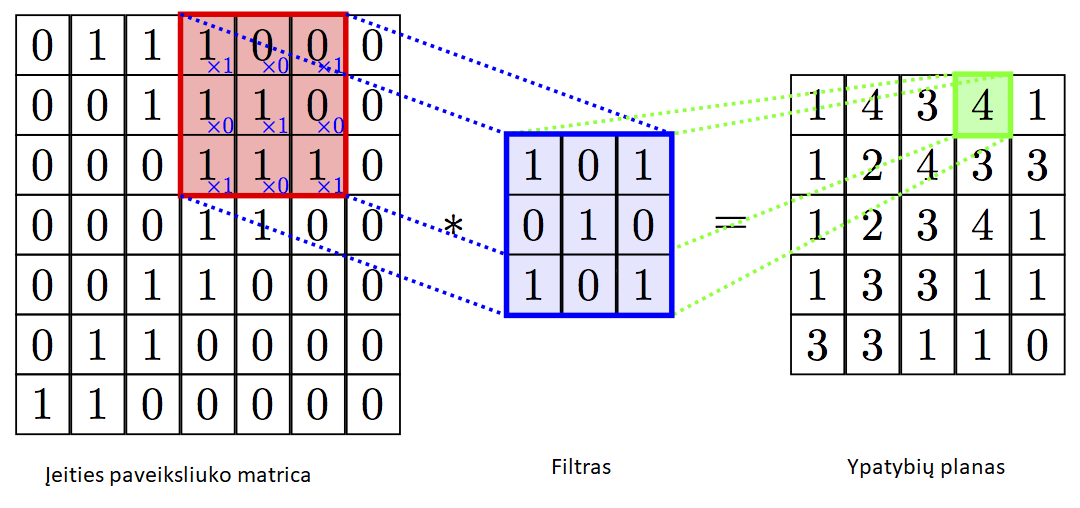
\includegraphics[width=0.5\textwidth]{img/Konvoliucija.png}
\caption{Konvoliucijos veikimas}
\end{figure}

Pagal paveiksliuką (1 pav.) matyti, kad įvesties duomenys ir filtras, kuris yra sudarytas iš svorių, yra pateikti 2D matrica. Filtras juda nuo duomenų matricos kairės viršutinės dalies į dešinę, 
tada yra nuleidžiamas žemiau per vieną eilutę ir taip filtras juda per visą duomenų matricą, kol su visais jos duomenimis filtras yra sudauginamas ir užpildo naują matricą, kuri 
yra vadinama ypatybių planu (angl. feature map).
Tačiau konvoliuciniai tinklai turi daug filtrų, kurie pereina per vieną paveiksliuką, kiekvienas išskirdamas skirtingą paveiksliuko ypatybę \cite{DBLP:journals/corr/abs-1708-08711}.
Pirmuose sluoksniuose šiuos filtrus galima apibūdinti kaip horizontalių, vertikalių ar įstrižų linijų filtrus, kurie sukuria paveikslėlio 
kraštų planą.

\subsection{Konvoliucinio neuroninio tinklo sluoksniai}
Konvoliuciniai neuroniniai tinklai tai yra sluoksnių rinkinys, kuris turi įvesties, vidinius ir išvesties sluoksnius. Tačiau priklausomai 
kokio tipo konvoliucinis neuroninis tinklas vidiniai sluoksniai gali skirtis. Konvoliuciniai neuroniniai tinklai turi tris pagrindinius 
sluoksnių tipus, kurie sudaro vidinį sluoksnį. Šie tipai yra konvoliucinis, sujungimo ir pilno sujungimo sluoksniai \cite{CNNbasic}.

Nepagrindinių sluoksnių paaiškinimai:
\begin{itemize}
\item Plokštinimo sluoksnis (angl. flatten layer) - skirtas tam, kad įeinančius duomenis suploti į atitinkamą sluoksnių skaičių, jeigu sluoksnio parametras nenustatytas suplojama į vieną sluoksnį.
\item Išmetimo sluoksnis (angl. dropout layer) - sluoksnyje atsitiktinai yra išjungiami tam tikri neuronai su Bernulio pasiskirstymo tikimybe, kuri priima dvi reikšmes 1 (sėkmė) ir 0 (nesėkmė) 
bei šių reikšmių tikimybe \(p\) ir \(1 - p\). Dažniausiai yra nustatytas 50 procentų.
\end{itemize}

\subsubsection{Konvoliucinis sluoksnis}
Konvoliucinis sluoksnis (angl. convolutional layer) yra pagrindinis konvoliucinio neuroninio tinklo sluoksnis, kuris nustato visas paveiksliuko ypatybes.
Kadangi įvesties informacija (paveiksliukas) yra didelės dimensijos, neefektyvu visų neuronų sujungti vienus su kitais, todėl neuronai yra sujungiami
su lokaliu informacijos kiekiu, kuris yra lygus filtro dydžiui ir vadinamas erdviniu mastu (angl. receptive field) \cite{layers-CS231n}.

Neuronų kiekis po konvoliucijos (ypatybių plano dydis) yra nustatomas trimis parametrais:
\begin{itemize}
\item Gylis (angl. depth) - atitinka filtrų skaičių.
\item Žingsnis (angl. stride) - pikselių kiekis, kuris parodo per kiek reikia slinkti filtro matrica per įvesties informacijos matricą.
\item Nulių pamušalas (angl. zero-padding) - įvesties informacijos matricos kraštus užpildyti nuliais.
\end{itemize}

\subsubsection{Sujungimo sluoksnis}
Periodiškai sujungimo sluoksnis (angl. pooling layer) yra įterpiamas tarp konvoliucinių. Pagrindinis sluoksnio tikslas yra laipsniškai mažinti erdvinį filtruojamo paveiksliuko mastą.
Šis veiksmas yra atliekamas tam, kad sumažinti parametrų ir skaičiavimų kiekį. Maksimumo sujungimo (angl. max pooling) sluoksnis, nepriklausomai nuo kiekvieno
sluoksnio gylio, yra erdviškai (ilgis ir plotis) keičiamas ir rezultatas gaunamas naudojant MAX operaciją \cite{7927440}. Dažnai šis sluoksnis yra naudojamas su 2x2 dydžio filtru - įvesties 
duomenys yra suskaidomi į keturias lygias dalis ir iš kiekvienos dalies paimama didžiausia tos dalies reikšmė, iš šių reikšmių sudaroma nauja matrica. Egzistuoja ne tik 
maksimumo sujungimo sluoksniai, bet ir vidurkio sujungimo (angl. average pooling) - jame yra randama ne didžiausia matricos dalies reikšmė, o suskaičiuojamas vidurkis.

\subsubsection{Pilno sujungimo sluoksnis}
Pilno sujungimo sluoksnis (angl. fully connected layer) yra sujungtas su visais 
neuronais iš sluoksnio buvusio prieš jį. Šio sluoksnio tikslas yra panaudojant tas ypatybes, kurios yra gautos iš prieš tai buvusių sluoksnių, nustatyti kokioms 
klasėms priklauso įvesties paveiksliukas pagal mokymo informacijos imtį, kai neuroninio tinklo problema yra klasifikacija \cite{layers-fullyconnected}. Šiam 
sluoksniui yra priskiriama aktyvacijos funkcija, kuri neprivalo būti tokia pati kaip vidiniuose sluoksniuose naudota aktyvacijos funkcija. 

\subsection{Architektūros}
Konvoliuciniai neuroniniai tinklai turi keletą skirtingų architektūrų, kurios naudojamos pagal sprendžiamą problemą. 1 lentelėje pateikta informaciją 
apie įvairias architektūras.

\begin{longtable}[h]{ | p{4cm} | p{1cm} | p{3cm} | p{5cm} | p{1.5cm} | } 
\caption{Konvoliucinių neuroninių tinklų architektūros}
\hline
Pavadinimas & Metai & Parametrų kiekis & Veikimas & ILSVRC vieta \\
\hline
\endhead
LeNet & 1998 & 60 000 & Geriausiai atpažįsta ranka parašytus skaičius. Susideda iš sluoksnių - kelių pasikartojančių konvoliucijos ir sujungimo bei pasibaigia dviem pilno sujungimo sluoksniais. & - \\
\hline
AlexNet & 2012 & 60 000 000 & Veikimu panašus į LeNet, tačiau turi daug daugiau parametrų ir filtrų bei sudėtus konvoliucinius sluoksnius.  & pirma \\
\hline
GoogLeNet/Inception & 2014 & 4 000 000 & Vidiniai sluoksniai sudėti paraleliai, naudojami Inception moduliai. Vienas modulis savyje turi 1x1, 3x3 ir 5x5 dydžių konvoliucijos filtrų bei vidurkio sudėjimo sluoksnius. & pirma \\
\hline
VGGNet & 2014 & 138 000 000 & Panašus veikimas į AlexNet, tačiau daug gilesnis. Naudojamų filtrų dydis yra 3x3 ir jie yra sudėti vienas po kito. & antra \\
\hline
ResNet & 2015 & 25 000 000 & Turi labai daug sluoksnių, sudėtų vienas po kito, kurie turi liekamąjį (angl. residual) bloką, kuris įvesties informaciją perduoda tolimesniam sluoksniui ją pridėdamas ir taip sumažina konvoliucijos ir aktyvavimo funkcijų kiekį.  & pirma \\
\hline
CUImage & 2016 & - & Dvipusis dvikryptis tinklas, kuris perduoda žinutes tarp skirtingų paramos regionų. & pirma \\
\hline
SENets & 2017 & 25 600 000 & Panašus veikimas į ResNet, pridėtas SE blokas, kuris sujungia ypatybių planus ir valdo išėjimus iš kanalo.  & pirma \\
\hline
\end{longtable}

\subsection{Modelio derinimas}
Apmokius neuroninį tinklą ir nustačius vidinių parametrų reikšmes gaunamas neuroninio tinklo architektūros modelis. Tokį jau egzistuojantį modelį galima derinti (angl. fine-tune) 
ir pritaikyti specifiniai užduočiai spręsti. Modelį derinti galima nustačius kelis paskutinius sluoksnius kaip mokomus (angl. trainable) ir su mažiau duomenų galima modelį suderinti.

Toks suderinimas yra galimas, nes pirmuosiuose sluoksniuose neuroniniai tinklai išmoksta ypatybių panašių į Gaboro filtrą 
(tiesinis filtras naudojamas tekstūroms analizuoti) ir spalvų dėmes. Šios pirmojo sluoksnio ypatybės nepriklauso nuo duomenų rinkinio, bet yra bendros ir tinkamos 
daugeliui duomenų rinkinių ir užduočių \cite{DBLP:journals/corr/YosinskiCBL14}.

\section{Technologijos}
Naudojamų technologijų išsirinkimas yra pradinis žingsnis siekiant įvykdyti kursiniame darbe išsikeltas užduotis. Šiame skyriuje pateiktos populiariausios šių laikų technologijos 
bei glaustai apibrėžti jų pagrindiniai funkcionalumai.

\subsection{ImageNet}
Projektas ImageNet buvo sugalvotas profesorės Li Fei-Fei 2009 metais. Projekto tikslas buvo sukurti didelę sukategorizuotų paveiksliukų ir jų etikečių duomenų bazę, 
kuri butų skirta vizualinio objekto atpažinimo programinės įrangos tyrimams. Ši duomenų bazė yra suorganizuota pagal WorldNet hierarchija - anglų kalbos žodžiai 
yra grupuojami į sinonimų rinkinius, kurie turi apibūdinimus ir naudojimo pavyzdžius bei saugo ryšių kiekį tarp sinonimų arba jų narių. ImageNet turi daugiau nei 
100 000 sinonimų rinkinių, kur didžioji dalis yra daiktavardžiai (80 000+). 

ImageNet projektas kiekvienais metais daro konkursą vadinamą "ImageNet Large Scale Visual Recognition Challenge" (trumpinys ILSVRC). Konkurso užduotis yra 
išmokinti modelį, kuris galėtų įvesties paveiksliuką teisingai klasifikuoti į 1000 skirtingų objektų klasių, kurios atitinka realius daiktus, gyvūnus ir t.t. Modeliai 
yra apmokomi su apie 1.2 milijonų paveiksliukų ir dar 50 000 paveiksliukų yra naudojami validacijai mokymo metu bei 100 000 paveiksliukų yra panaudojami galutiniam 
modelio testavimui. Šis konkursas yra paveiksliukų klasifikacijos algoritmų etalonas.

\subsection{Keras}
Keras yra aukšto lygio programų sąsaja skirta neuroniniams tinklams. Sąsaja parašyta su Python programavimo kalba ir vidinėje pusėje galinti veikti su "TensorFlow" 
ir kitomis bibliotekomis. Keras buvo sukurtas tikintis suteikti greitą eksperimentavimą, kad sugalvojus idėją pasiekti rezultato būtų galima su kiek įmanoma mažiau uždelsimo.

Ši sąsaja savyje turi visus pagrindinius neuroninio tinklo kūrimo blokus, pavyzdžiui, sluoksniai, aktyvavimo ir optimizavimo funkcijos. Taip pat Keras suteikia modelius, 
kurie yra apmokyti naudojant ImageNet duomenų bazę. Šiuos modelius galima derinti, pridėti papildomų sluoksnių, pasirinkti esamus sluoksnius bei juos iš naujo apmokyti.

\subsection{TensorFlow}
TensorFlow yra atviros programinės įrangos biblioteka skirta aukšto našumo skaitiniams skaičiavimams. Jo lanksti architektūra leidžia lengvai diegti skaičiavimus įvairiose 
platformose - procesoriuose, grafikos procesoriuose. Sukurtas "Google" dirbtinio intelekto skyriaus, tad yra labai palaikomas automatinis ir gilusis mokymasis, tačiau 
dėl bibliotekos ir skaičiavimų lankstumo yra naudojamas įvairiose mokslinėse srityse.

\section{Eksperimentas}
Šio eksperimento tikslas yra išanalizuoti mokymosi tikslumą su skirtingų gylių neuroninais tinklais, kai mokymui yra naudojamas mažas paveikslėlių rinkinys. Taigi, pirmas 
šio eksperimento žingsnis - išsirinkti konvoliucinį neuroninį tinklą. Poskyriuje "Architektūros" yra trumpai apibūdinti pagrindiniai konvolicinių neuroninių tinklų tipai. 
Iš jų buvo išsirinktas VGG, kadangi jis neturi specialių blokų kaip kad GoogleNet turi inception arba ResNet turi liekamąjį, todėl yra paprasta suvokti kaip duomenys sklinda per tinklą. Buvo nuspręsta daryti paprastą, binarinę paveikslėlių 
klasifikaciją - nustatymas ar katė, ar šuo pavaizduotas paveikslėlyje. Buvo surasta ir naudota duomenų imtis, kuri turi 10 000 paveikslėlių - 8 000 mokymosi tikslui ir 2 000 validacijos.

% \subsection{Duomenų rinkinys}
% Tinklas turi aukščiausią tikslumą, kai yra apmokomas su bendriniais duomenimis ir dar efektyviau 
% pasirodo kai yra suderintas su specifiniu duomenų rinkiniu \cite{DBLP:conf/eccv/ChuMBHD16}. Optimalus duomenų kiekis, kad gerai suderinti 
% modelį yra apie 10 000 paveiksliukų. 
% Tačiau realybėje visų klasių objektų paveiksliukų nėra be galo daug, kadangi reikia turėti daug paveiksliukų ir skirti labai
% daug laiko bei žmogiškųjų resursų jų žymėjimui. Todėl tenka tinklus apmokyti su limituotais duomenų rinkiniais. Pagal šią realaus pasaulio problemą buvo įvykdyta viena iš eksperimento tikslo sąlygų - 
% mažas duomenų rinkinys. Buvo surasta ir naudota duomenų imtis, kuri turi 10 000 paveikslėlių - 8 000 mokymosi tikslui ir 2 000 validacijos.

\subsection{Programos veikimas}
Ankstesniame skyriuje "Technologijos" yra išvardintos visos technologijos, kurios buvo naudotos šio eksperimento programai parašyti.

Ruošiantis eksperimentui reikia paruošti kompiuterį darbui - įrašyti "Python" programavimo įrankius, paruošti "Anaconda" komandinę eilutę, "NVIDIA CUDA" įrankius, Keras ir 
TensorFlow. Tačiau kompiuteris privalo turėti tinkamą procesorių ar grafinį procesoriaus bloką - kompiuteris, kurį naudojau turėjo Nvidia 1080 Ti. Programa, kuri 
derina modelį ir modifikuoja, nelabai skiriasi, tad modelio derinimo eiga buvo vėliau pritaikyta ir modifikavimo daliai. 
 
Keras pateikia modelius, apmokytus su ImageNet, ir jų svorius, tad reikia tik importuoti 
tinkamą modelį - šiuo atveju VGG16. Importavimo metu reikia nustatyti, kad pilnai sujungtas sluoksnis nebūtų pridėtas, kadangi tada galima parinkti kokių dimensijų 
paveiksliukai naudojami ir kiek spalvų sluoksnių jie turi (standartiniai paveiksliukai turi 3). Tuomet reikia nustatyti kokius importuoto modelio sluoksnius norima 
mokinti ir kuriuos - ne. Iš visų esamų sluoksnių mokinimui buvo parinkti tik paskutiniai 4, kadangi jie yra atsakingi už specifinių ypatybių išmokimą. Po šių egzistuojančio 
modelio paruošimų reikia sukurti naują Kero modelį, prie kurio reikia pridėti paruoštą egzistuojantį modelį bei pridėti kelis kitus sluoksnius tam tikru išsidėstymu - 
plokštinimo (angl. flatten), tankumo (angl. dense), išmetimo (angl. dropout) ir vėl tankumo. Pirmasis tankumo sluoksnis turi aktyvacijos funkciją ReLU, o paskutinis - sigmoidinę. Po visų sluoksnių pridėjimo modelis iš 
viso turėjo 40 406 849 parametrų, iš kurių mokinami buvo 32 771 585, o tik 7 635 264 buvo nekeičiami. 

Po modelio paruošimo, reikia nustatyti kokio dydžio paveikslėlių partijomis (angl. batch) bus mokomas ir validuojamas modelis. Geriausias partijos dydis naudotam kompiuteriui buvo mokymosi partijai 100 paveikslėlių, o validacijos - 25.
Tuomet nustatomas paveikslėlių aplankalo kelias, jų ir partijos dydis bei nustatomas klasės režimas į binarinį, nes duomenų rinkinys susideda iš dviejų klasių - kačių ir šunų.

Paruošę modelį bei paveikslėlių rinkinį, galima pradėti mokinti ir validuoti modelį. Taigi, nustatomas modelio kompiliavimo metodas, kur turi būti - nuostolio ir 
optimizavimo funkcijos. Daugiau apie nuostolio ir optimizavimo funkcijas galima skaityti skyriuose "Nuostolio funkcijos" ir "Optimizavimo funkcijos". Tačiau nuotolio 
funkcija šiame modelyje yra binarinė kryžiaus entropija, kuri nebuvo keičiama. Šio eksperimento metu bus naudojamos keturios optimizavimo funkcijos - SGD, 
Adam, Adagrad ir RMSprop. Po modelio sukompiliavimo yra aprašomas mokymo metodas, kuriam turi būti pateikta - paruošti paveiksliukai, žingsnis per epochą, epochų kiekis, 
paruošti validacijos paveiksliukai ir jų žingsnis. Taigi, šiame eksperimente epocha yra nustatyta 80, kadangi tokia išeina pagal visų turimų paveiksliukų skaičių ir paketo dydį.

Modelio modifikavimo veikimas yra toks pats išskyrus, kad pridedami ne 4 sluoksniai, o 14 sluoksnių, kurie visi yra tankumo sluoksniai su aktyvacijos funkcija ReLu. Jie yra 
pridedami tarp plokštinimo ir kito tankumo sluoksnio. Po visų sluoksnių pridėjimo iš viso buvo 51 952 449 parametrų, iš kurių buvo 44 317 185 mokinami, o tiek pat buvo nemokinami 
kaip ir derinant modelį. Taigi, modifikavimo metu prisidėjo papildomi 11 545 600 parametrų.

\subsection{Modelių mokymas}
Parašius programas, kurios derina bei modifikuoja modelį, buvo pradėta jį mokyti ir validuoti su skirtingomis optimizavimo funkcijomis.
Mokymosi greitis buvo išrinktas 1e-4, kas yra 0.0001.
\subsubsection{Modelio derinimas}
Pasirinkta buvo pradėti eksperimentą nuo modelio modifikavimo, kadangi tokiu būdu galima pamatyti kaip modelio paskutiniai keli sluoksniai yra apmokomi ir kaip tikslumas ir nuostolis 
keičiasi mokymo metu, kai yra naudojamas negilus modelis.

Taigi, pirmiausiai buvo pasirinkta SGD optimizavimo funkcija. Apmokius modelį buvo gauti grafikai - 3 ir 4 paveiksliukai.

\begin{figure}[!htbp]
  \centering
  \begin{minipage}[b]{0.49\textwidth}
    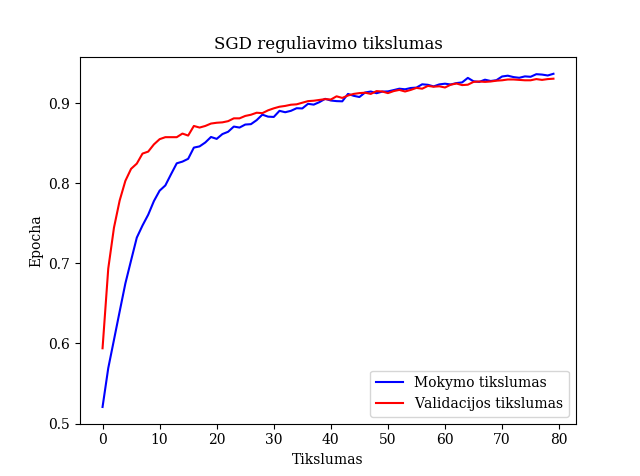
\includegraphics[width=\textwidth]{img/FT/SGD_acc.png}
    \caption{Modelio mokymosi ir validacijos tikslumas naudojant SGD}
  \end{minipage}
  \begin{minipage}[b]{0.49\textwidth}
    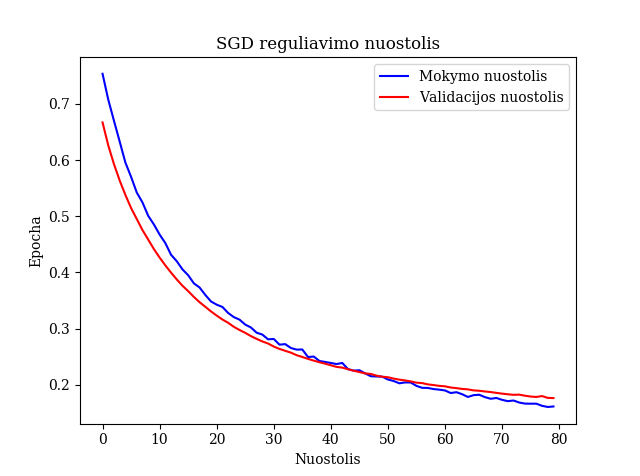
\includegraphics[width=\textwidth]{img/FT/SGD_loss.png}
    \caption{Modelio mokymosi ir validacijos nuostolis naudojant SGD}
  \end{minipage}
\end{figure}

Grafikas (3 pav.) parodo, kad tikslumas kyla kuo daugiau modelis išmoksta ir validacijos funkcija pirmiausiai pranoksta mokymosi, bet vėliau susilygina. Aukščiausias tikslumo rezultatas yra apie 94 procentus.
Grafikas (4 pav.) rodo nuostolį per epochas. Iš jo matoma, kad mokymosi ir validacijos nuotoliai ties 47 epocha susikerta ir validacijos nuostoliai tampa didesni už mokymosi.

Vėliau keičiama optimizavimo funkcija į Adam - mokymosi rezultatai matomi grafikuose - 5 ir 6 paveiksliukuose.

\begin{figure}[!htbp]
  \centering
  \begin{minipage}[b]{0.49\textwidth}
    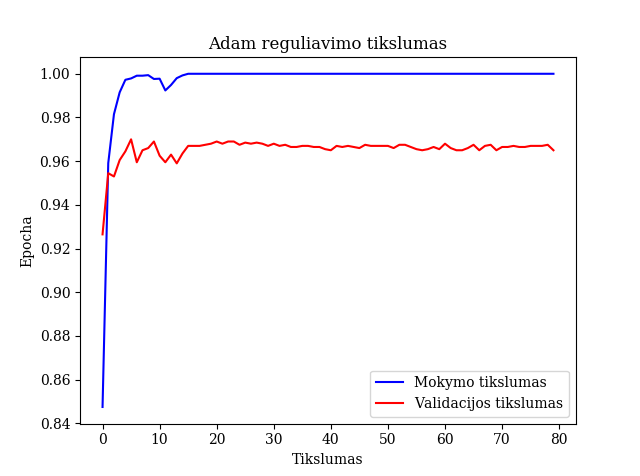
\includegraphics[width=\textwidth]{img/FT/Adam_acc.png}
    \caption{Modelio mokymosi ir validacijos tikslumas naudojant Adam}
  \end{minipage}
  \begin{minipage}[b]{0.49\textwidth}
    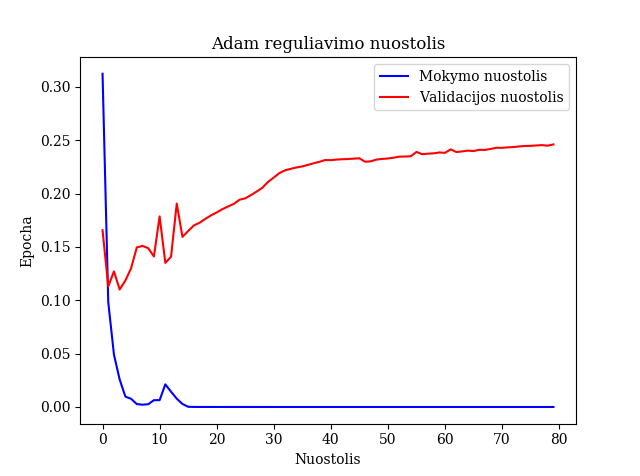
\includegraphics[width=\textwidth]{img/FT/Adam_loss.png}
    \caption{Modelio mokymosi ir validacijos nuostolis naudojant Adam}
  \end{minipage}
\end{figure}

Tikslumo grafikas (5 pav.) parodo, kad mokymosi tikslumas per kelias pirmas epochas pasiekia beveik 100 procentinį tikslumą, tačiau validacijos lieka apie 96 procentus ir daugiau nebekyla.
O nuostolio grafikas (6 pav.) parodo, kad mokymosi nuostolis staigiai nukrenta iki beveik 0 procentų nuostolių. Tačiau validacijos nuostoliai per kelias epochas nukrenta, o po to staigiai pradeda augti ir išsilygina ties 24 procentais.

Trečiasis testuojama optimizavimo funkcija yra Adagrad. Jos grafikai yra 7 ir 8 paveiksliukai.

\begin{figure}[!htbp]
  \centering
  \begin{minipage}[b]{0.49\textwidth}
    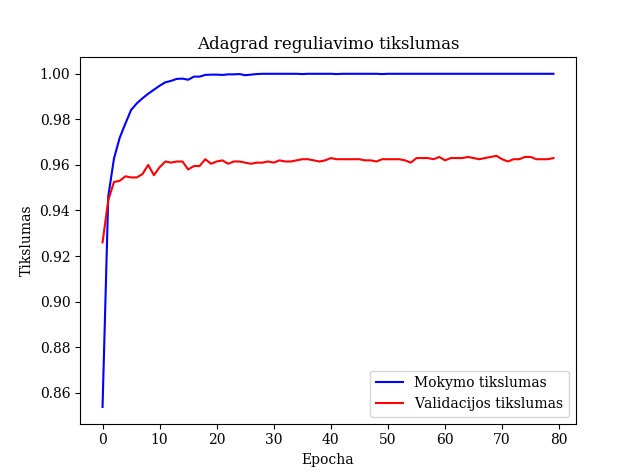
\includegraphics[width=\textwidth]{img/FT/Adagrad_loss.png}
    \caption{Modelio mokymosi ir validacijos tikslumas naudojant Adagrad}
  \end{minipage}
  \begin{minipage}[b]{0.49\textwidth}
    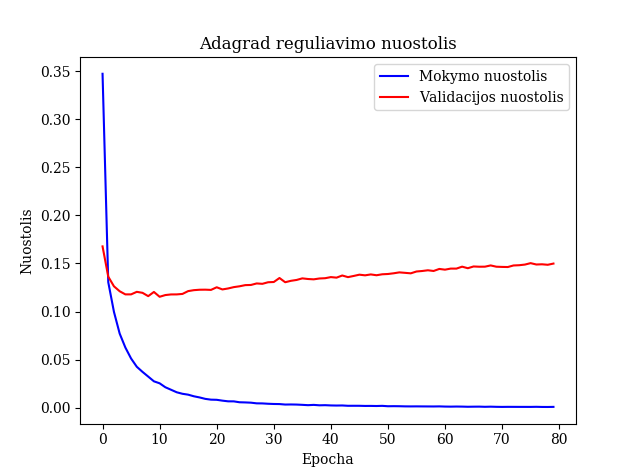
\includegraphics[width=\textwidth]{img/FT/Adagrad_acc.png}
    \caption{Modelio mokymosi ir validacijos nuostolis naudojant Adagrad}
  \end{minipage}
\end{figure}

Galima daryti išvadą, jog tikslumo grafikas (7 pav.) parodo, kad mokymosi tikslumas per pirmas 20 epochų pakyla beveik iki 100 procentų, o validacijos tikslumas pakyla iki 96 procentų ir ties tiek pasilieka.
O nuostolio grafikas (8 pav.) parodo, kad taip pat kaip ir mokymosi tikslumas taip ir nuostolis per pirmas 20 epochų nukrenta iki beveik 0 procentų ir ties ten lieka. Kai validacijos nuostolis 
nukrenta iki tolygiai auga iki 11 procentų, o po to tolygiai kyla iki 15 procentų.

Paskutinis bandymo optimizavimo funkcija yra RMSprop. Ji yra parodyta 9 ir 10 paveiksliukuose.

\begin{figure}[!htbp]
  \centering
  \begin{minipage}[b]{0.49\textwidth}
    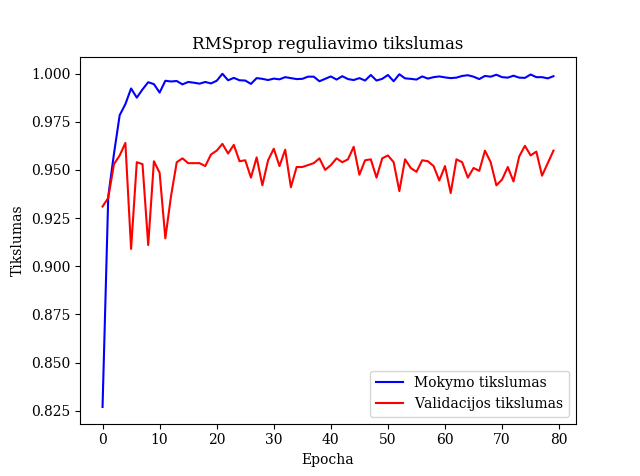
\includegraphics[width=\textwidth]{img/FT/RMSprop_acc.png}
    \caption{Modelio mokymosi ir validacijos tikslumas naudojant RMSprop}
  \end{minipage}
  \begin{minipage}[b]{0.49\textwidth}
    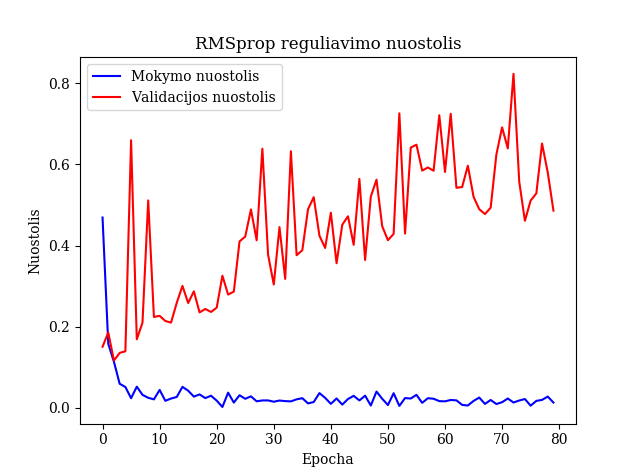
\includegraphics[width=\textwidth]{img/FT/RMSprop_loss.png}
    \caption{Modelio mokymosi ir validacijos nuostolis naudojant RMSprop}
  \end{minipage}
\end{figure}

Tad, tikslumo grafikas (9 pav.) parodo, kad mokymosi funkcija šokteli iki 100 procentų ir ten išsilaiko, kai validacijos funkcija stipriai svyruoja tarp 93 ir 95 procentų, bet per visas epochas neišsilygina.
O nuostolio grafikas (10 pav.) parodo, kad mokymosi funkcija nukrenta iki beveik 0 procentų ir ten išsilaiko. Tačiau validacijos funkcija labai stipriai svyruoja ir didėja. Pasiekdama aukščiausią nuostolį ties 82 procentais.

\subsubsection{Modelio modifikavimas}
Iš naujo apmokyti modeliai su 14 papildomų sluoksnių. Visi parametrai ir duomenų rinkinys liko tokie patys tik optimizavimo funkcija vėl buvo keičiama.

Kaip ir prieš tai pirmoji modifikavimo funkcija yra SGD. Jos grafikai yra 11 ir 12 paveiksliukai.

\begin{figure}[!htbp]
  \centering
  \begin{minipage}[b]{0.49\textwidth}
    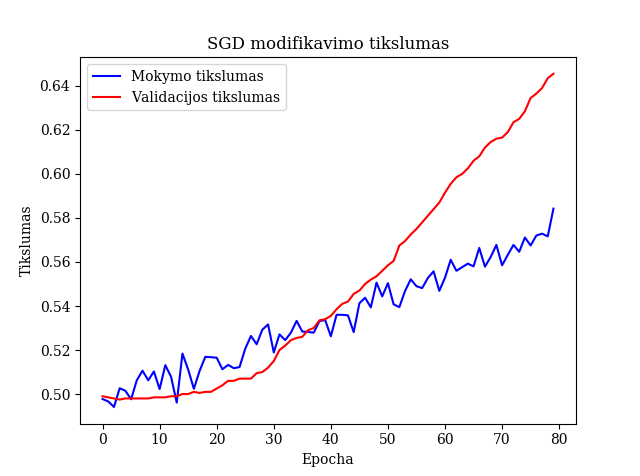
\includegraphics[width=\textwidth]{img/AL/SGD_acc.png}
    \caption{Gilesnio modelio mokymosi ir validacijos tikslumas naudojant SGD}
  \end{minipage}
  \begin{minipage}[b]{0.49\textwidth}
    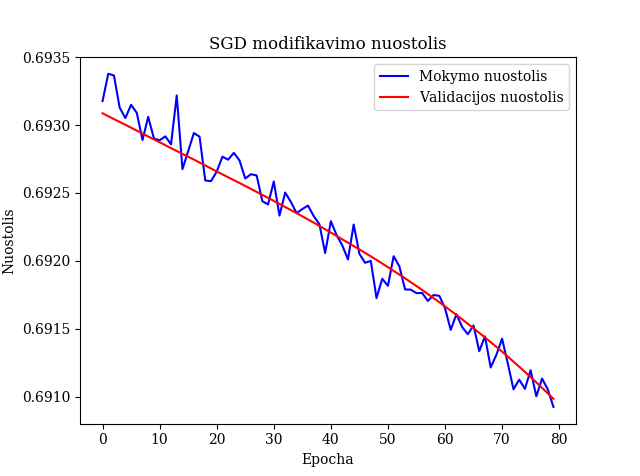
\includegraphics[width=\textwidth]{img/AL/SGD_loss.png}
    \caption{Gilesnio modelio mokymosi ir validacijos nuostolis naudojant SGD}
  \end{minipage}
\end{figure}

Tikslumo grafikas (11 pav.) matyti, kad mokymosi funkcija tolygiai svyruojančiai didėja, tačiau validacijos tikslumas ties 37 epocha pranoksta mokymosi bei pati validacijos funkcija tolygiai kyla ir neturi 
tokių svyravimų kaip mokymosi. Palyginus su 3 paveiksliuko tikslumu, po papildomų sluoksnių pridėjimo nei validacijos nei mokymosi tikslumas nepasiekia tokio aukšto tikslumo, koks buvo mažesnio gylio modelyje.
Nuostolio grafike (12 pav.) parodyta, kad mokymosi ir validacijos funkcijos tolygiai mažėja, tačiau mokymosi svyruoja. Tačiau mažiausias nuostolis šiame grafike yra 69 procentai, kai 4 paveiksliuke, kur parodyta 
ne tokio gilaus modelio nuostoliai, mažiausi pasiekti nuostoliai yra 20 procentų.

Antra bandoma optimizavimo funkcija yra Adam. Jos grafikai yra 13 ir 14 paveiksliukai.

\begin{figure}[!htbp]
  \centering
  \begin{minipage}[b]{0.49\textwidth}
    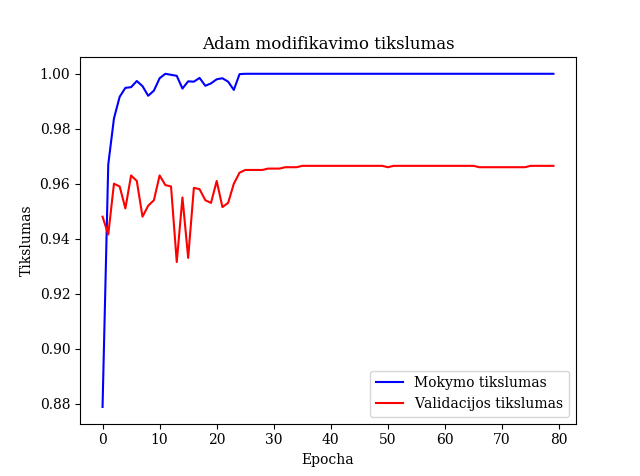
\includegraphics[width=\textwidth]{img/AL/Adam_acc.png}
    \caption{Gilesnio modelio mokymosi ir validacijos tikslumas naudojant Adam}
  \end{minipage}
  \begin{minipage}[b]{0.49\textwidth}
    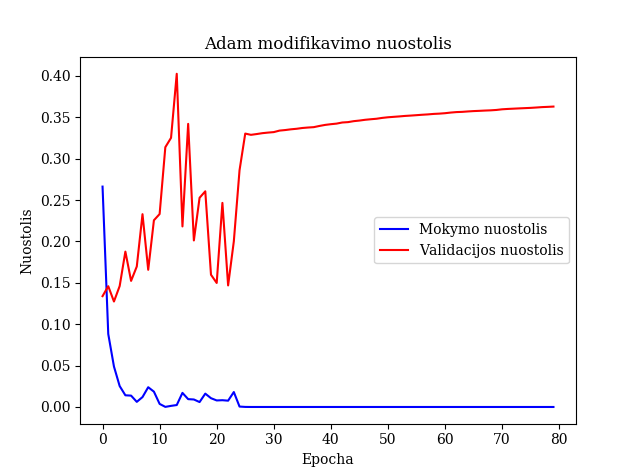
\includegraphics[width=\textwidth]{img/AL/Adam_loss.png}
    \caption{Gilesnio modelio mokymosi ir validacijos nuostolis naudojant Adam}
  \end{minipage}
\end{figure}

Tikslumo grafiką (13 pav.) palyginus su 5 paveiksliuku matyti, kad mokymosi tikslumo funkcija pakilo iki 100 procentų, panašiu greičiu. Validacijos funkcija gilesniame modelyje pirmose 25 epochų ganėtinai 
stipriai svyravo, tačiau po to išsilygino ties 96 procentais. 
Tačiau nuostolio grafikas (14 pav.) labai skiriasi nuo 6 paveiksliuko, kur parodyta ne tokio gilaus modelio nuostolis. Mokymosi funkcija kaip ir mažesnio gylio modelio mažėja iki 0 procentų, tačiau validacijos nuostolis 
daug stipriau svyruoja pirmose 25 epochose, o po to išsilygina ir pradeda tolygiai didėti, pasiekdama didžiausia nuostolį ties 36 procentais.

Prieš paskutinė funkcija yra Adagrad. Šios funkcijos grafikai yra 15 ir 16 paveiksliukai.

\begin{figure}[!htbp]
  \centering
  \begin{minipage}[b]{0.49\textwidth}
    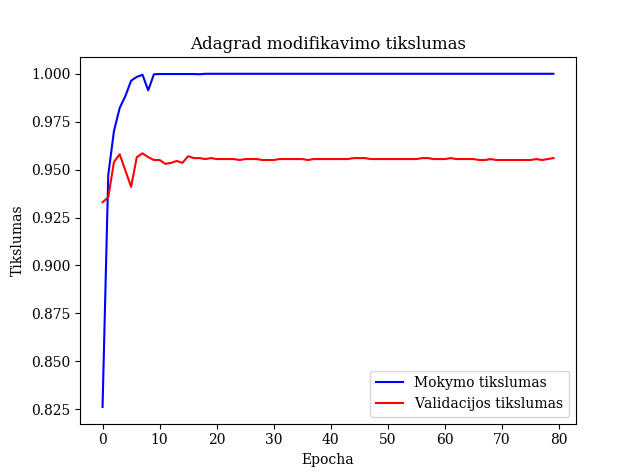
\includegraphics[width=\textwidth]{img/AL/Adagrad_acc.png}
    \caption{Gilesnio modelio mokymosi ir validacijos tikslumas naudojant Adagrad}
  \end{minipage}
  \begin{minipage}[b]{0.49\textwidth}
    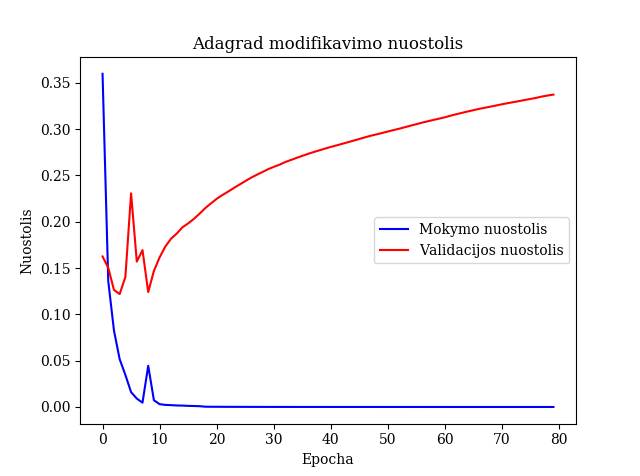
\includegraphics[width=\textwidth]{img/AL/Adagrad_loss.png}
    \caption{Gilesnio modelio mokymosi ir validacijos nuostolis naudojant Adagrad}
  \end{minipage}
\end{figure}

Tikslumo grafikas (15 pav.) yra labai panašus į mažesnio gylio tikslumo grafiką (7 pav.), kadangi mokymosi tikslumo funkcijos yra beveik vienodos, o validacija šiuo atveju yra šiek tiek mažesnio tikslumo gilesniame 
modelyje - susilygina ties 95 procentais.
Nuostolio grafikas (16 pav.) kaip ir 8 paveiksliuke, parodo, kad mokymosi nuostolis staigiai mažėja iki 0 procentų. O validacijos nuostolis pirmose 10 epochų stipriai svyruoja ir po to sparčiai auga ir pasiekia maksimalią nuostolio 
reikšmę ties 34 procentais, kai mažesnio gylio modelio yra apie 15 procentų.

Paskutinė optimizavimo funkcija yra RMSprop. Jos grafikai yra 17 ir 18 paveiksliukai.

\begin{figure}[!htbp]
  \centering
  \begin{minipage}[b]{0.49\textwidth}
    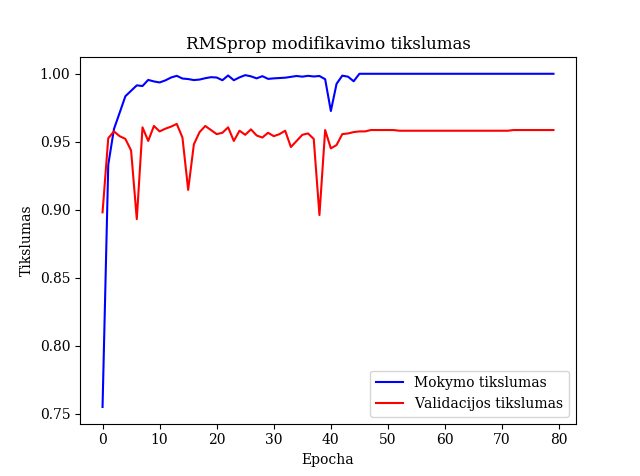
\includegraphics[width=\textwidth]{img/AL/RMSprop_acc.png}
    \caption{Gilesnio modelio mokymosi ir validacijos tikslumas naudojant RMSprop}
  \end{minipage}
  \begin{minipage}[b]{0.49\textwidth}
    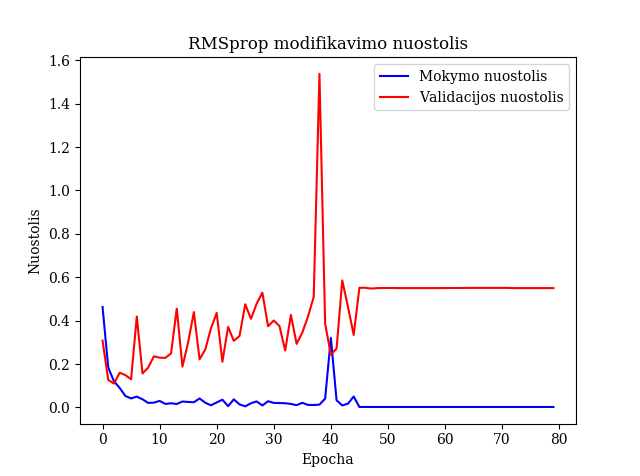
\includegraphics[width=\textwidth]{img/AL/RMSprop_loss.png}
    \caption{Gilesnio modelio mokymosi ir validacijos nuostolis naudojant RMSprop}
  \end{minipage}
\end{figure}

Tikslumo grafike (17 pav.) matyti, kad mokymosi funkcija pakyla iki 100 procentų, o validacijos funkcija svyruoja iki 40 epochos, o po to išsilygina ties 95 procentais, kai toks pat rezultatą matomas ir 9 paveikslėlyje, kuriame parodyta mažiau gilaus modelio tikslumas.
Nuostolio grafikas (18 pav.) parodo, kad mokymosi funkcija pasiekia 0 procentų. Tačiau validacijos funkcija svyruoja pirmas 45 epochas, o po to išsilygina ties 55 procentais.

\sectionnonum{Rezultatai ir išvados}
Darbo rezultatai:
\begin{enumerate}
\item Buvo atlikta bendra dirbtinių neuroninių tinklų ir konvoliucinių neuroninių tinklų analizė.
\item Egzistuojantis modelis buvo suderintas su pasirinkta kačių ir šunų duomenų imtimi.
\item Egzistuojantis modelis buvo modifikuotas, pridėjus papildomus 14 sluoksnių, ir suderintas su kačių ir šunų duomenų imtimi.
\item Gauti suderinto ir modifikuoto-suderinto modelių mokymo ir validacijos tikslumo grafikai.
\item Suderinimo metu buvo keičiamos optimizavimo funkcijos - iš viso panaudotos SGD, Adam, Adagrad ir RMSprop funkcijos, kurios buvo palyginus naudojantis mokymo ir validacijos grafais.
\end{enumerate}

\hfill\break

Darbo išvados:
\begin{enumerate}
\item Apmokius skirtingų gylių neuroninius tinklus, buvo nustatyta, kad gilesnis tinklas mokomojoje dalyje pasirodo labai gerai - tikslumas auga ir nuostolis mažėja iki 0 procentų, tačiau 
validacijos metu tikslumas pakyla iki tam tikros reikšmės ir pasidaro pastovus, o praradimas tolygiai auga. Galima daryti išvadą, kad gilesnis neuroninis tinklas su mažu kiekiu duomenų gali juos 
įsiminti, o ne išmokti atpažinti.
\item Atliktas eksperimentas parodė, kad su naudota duomenų imtimi ir parametrais, mažo gylio modeliuose geriausia naudoti Adagrad optimizavimo funkciją, kadangi jos pasiektas validacijos tikslumas yra 96 procentai, nors ir Adam funkcija pasiekė tokį 
patį tikslumą. Tačiau Adam funkcijos validacijos nuostolis 80 epochoje siekė 25 procentus, kai Adagrad siekė tik 15 procentų ir augimo tendencija buvo daug mažesnė. Šiuo atveju, Adagrad funkcija yra geriau, kadangi ji pritaiko mokymosi greitį pagal 
parametrus - maži pakeitimai (žemas mokymosi greitis) prametrams, kurie pasikartoja dažnai, ir dideli pakeitimai (aukštas mokymosi greitis), kai parametrai nėra dažni. Todėl ši funkcija labai gerai pasirodo su maža duomenų imtimi \cite{2016arXiv161106652K}.
\item Eksperimentas parodė, kad su naudota duomenų imtimi ir parametrais, didesnio gylio modeliuose geriau naudoti Adam optimizavimo funkciją, kadangi validacijos tikslumas yra 96 procentai, o nuostolio funkcija pasiekia 35 procentus. O Adagrad 
funkcija pasiekia tikslumą 95 procentų ir nuostolį 35 procentų, tačiau turi labai didelę augimo tendenciją. Adam funkcija yra geriau, nes kaip ir Adagrad apskaičiuoja ir saugo mokymosi greitį kiekvienam parametrui, bet ir fiksuoja momento (angl. 
momentum) pasikeitimus, kas leidžia greičiau surasti lokalų minimumą ir konverguoti. Todėl su dideliu kiekiu parametrų veikia Adam geriau \cite{DBLP:journals/corr/KingmaB14}.
\end{enumerate}

\printbibliography[heading=bibintoc] 

\end{document}


